  {\color{teal!90}\chapter{Changing Boot Animation}\label{cap:changing-boot-animation}}

  \AddToShipoutPictureBG*{%
    \AtPageUpperLeft{%
      \raisebox{-\height}{%
        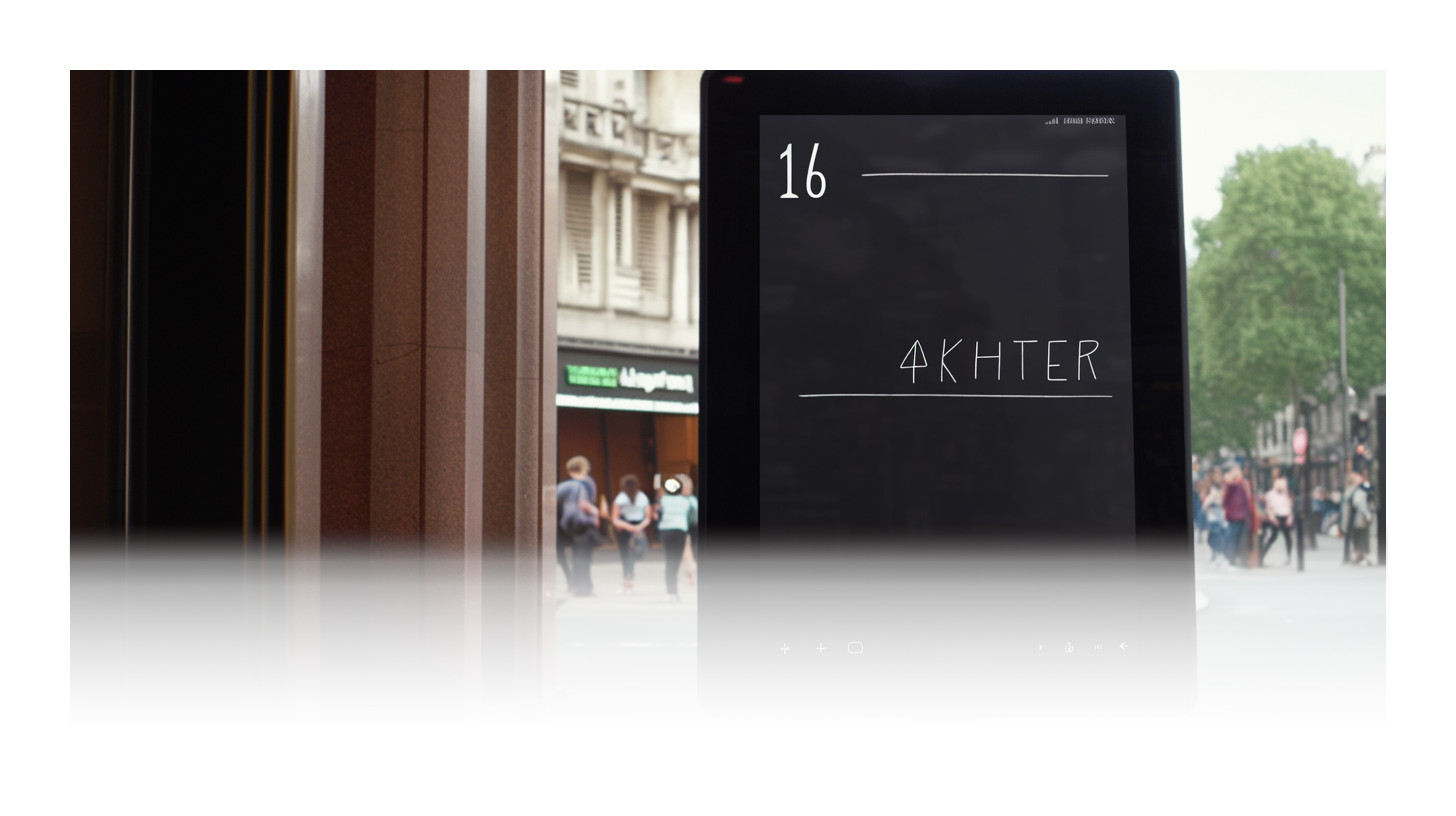
\includegraphics[width=\paperwidth]{./chapters/ifp_piccadilly.jpeg}%
      }%
    }
  }

  \minitoc% Creating an actual minitoc mini lista contenuti

  \section{Introduction}

  In this chapter, we will cover the steps required to customize the boot animation on a \gls{userdebug} device. This process involves creating a new boot animation, packaging it correctly, and using ADB commands to deploy it onto the device.

  \section{Creating the Boot Animation}

  The boot animation consists of multiple frames and a description file. For our device at Akhter Computers, the flat panel supports a maximum resolution of 2028x1126. The animation is generated in Blender and is divided into three parts:

  \begin{itemize}
    \item 81 frames in
    \begin{tikzpicture}[baseline=(text.base)]
      \node (icon) at (0, 0.3) {\color{Gray}\faIcon{folder-open}};
      \node (text) at (0, 0) {\desktopfile{akhter}};
    \end{tikzpicture}
    namely from 0 to 80. The first is called \desktopfile{fair\_00000.jpg} and the last \desktopfile{fair\_00080.jpg}

    \item 80 frames in
    \begin{tikzpicture}[baseline=(text.base)]
      \node (icon) at (0, 0.3) {\color{Gray}\faIcon{folder-open}};
      \node (text) at (0, 0) {\desktopfile{part1}};
    \end{tikzpicture}
    from 81 to 160. The first is called \desktopfile{00081.jpg} and the last \desktopfile{00160.jpg}

    \item A description in
    \begin{tikzpicture}[baseline=(text.base)]
      \node (icon) at (0, 0.3) {\color{Gray}\faIcon{file-alt}};
      \node (text) at (0, 0) {\desktopfile{desc.txt}};
    \end{tikzpicture}
    (cf. \ref{subsec:desc-txt})
  \end{itemize}

  The naming convention of the files seems to be very much free to choose in my opinion. The only requirement is that the files should be named in numerical order. The \desktopfile{desc.txt} file is used to manage the playback of the frames.

  \subsection{Description File - desc.txt}
  \label{subsec:desc-txt}

  The \emph{desc.txt} is managing the playback of the frames. This file is structured as follows:

  \begin{verbatim}
    2028 1126 30
    p 1 2 akhter
    p 0 0 part1
  \end{verbatim}

    \begin{itemize}
        \item `2028 1126 30`: Specifies the width, height, and \gls{fps} of the animation.
        \item `p 1 2 akhter`: Plays the frames in the "akhter" folder 1 time, with a 2-frame pause between loops.
        \item `p 0 0 part1`: Plays the frames in the "part1" folder indefinitely with no pause.
    \end{itemize}

  \subsection{Compressing the Boot Animation}

  To ensure the animation is displayed correctly, the compression factor must be set to 1.00. Use the following command to create the `bootanimation.zip`:


  \cmd{zip -r0 ./bootanimation.zip .}

  \section{Deploying the Boot Animation}

  Deploying the boot animation requires several ADB commands. This has been tested only on a \gls{userdebug} distro of Android.

  \subsection{Instructions \faCode}

  \begin{enumerate}
    \item Enable root access:

    \cmd{\faIcon{caret-right} adb root}

    \item Remount the system partition to make it writable:

    \cmd{\faIcon{caret-right} adb remount}

    \item Backup the existing boot animation:

    \cmd{\faIcon{caret-right} adb shell mv /product/media/bootanimation.zip /product/media/bootanimation.old.zip}

    \item Push the new boot animation to the device:

    \cmd{\faIcon{caret-right} adb push ./bootanimation.zip /product/media/bootanimation.zip}

    \item Sync the file system to ensure all changes are written:

    \cmd{\faIcon{caret-right} adb shell sync}
  \end{enumerate}
  \section{Conclusion}

  Customizing the boot animation on a userdebug device involves creating the animation frames, packaging them correctly, and using ADB commands to deploy the new animation. By following these steps, you can personalize the boot experience of your device.


%  \roundedwrap{19}{R}{0cm}{10cm}{./chapters/kioskTest_idea.png}{-10pt}{Kiosk Test Idea}{fig:kiosk-test-idea}{Black}
